%%%%%%%%%%%%%%%%%%%%%%%%%%%%%%%%%%%%%%%%%%%%%%%%%%%%%%%%%%%%%%%%%%%%%%%%
%%%%%%%%%%%%%%%%%%%%%% IMPORTANT %%%%%%%%%%%%%%%%%%%%%%%%%%%%%%%%%%%%%%%
%%%%%%%%%%%%%%%%%%%%%%%%%%%%%%%%%%%%%%%%%%%%%%%%%%%%%%%%%%%%%%%%%%%%%%%%
% Pour plus de clarté et de facilité pour votre rédaction              %
% veillez prendre en considération les bonnes pratiques                %
% suivantes :                                                          %
%                                                                      %
%   - Séparer les chapitres en fichiers distincts                      %
%   - Mettre les figures en sous dossiers                              %
%   - Utiliser un générateur de tableaux latex pour vos tableaux       %
% ( https://www.tablesgenerator.com/ )                                 %
%   - Dans le fichier de la bibliographie, toujours télécharger        %
% le code Bibtex des citations à partir des sites qui fournissent      %
% la publication.                                                      %
%   - N'hésitez pas à commenter les commandes latex que vous utilisez  %
%                                                                      %
% Ce template Latex est disponible sur le Github à l'adresse suivante: %
%   https://github.com/laiman-lab/tex-template                         %
% N'hésitez pas à l'améliorer et le distribuer.                        %
%                                               Bon travail            %
%                                               Aymen Goubaa           %
%%%%%%%%%%%%%%%%%%%%%%%%%%%%%%%%%%%%%%%%%%%%%%%%%%%%%%%%%%%%%%%%%%%%%%%%
%%%%%%%%%%%%%%%%%%% Début de la configuration %%%%%%%%%%%%%%%%%%%%%%%%%%
%%%%%%%%%%%%%%%%%%%%%%%%%%%%%%%%%%%%%%%%%%%%%%%%%%%%%%%%%%%%%%%%%%%%%%%%

\documentclass[12pt,a4paper]{report} 
\usepackage[utf8]{inputenc}
\usepackage[frenchb]{babel}
\usepackage{lipsum}
\usepackage{graphicx}
\usepackage{float}
\usepackage{url}
\usepackage{setspace}
\doublespacing
\usepackage{tikz}
\def\checkmark{\tikz\fill[scale=0.4](0,.35) -- (.25,0) -- (1,.7) -- (.25,.15) -- cycle;}%Rajoute une commande pour pouvoir insérer le signe "check" 
%espacement entre les lignes
\usepackage{setspace}
%modifier la mise en page de l'abstract
\usepackage{abstract}
%police et mise en page (marges) du document
\usepackage[T1]{fontenc}
\usepackage[top=2.5cm, bottom=2.5cm, left=2.5cm, right=2.5cm]{geometry} %Marges de la page  
\setcounter{secnumdepth}{4}% Profondeur de la table des matières
\setcounter{tocdepth}{4}% Profondeur de la table des matières
\usepackage{hyperref} % pour integrer les liens interne au pdf (table matières, figures, références ... cliquables)
\renewcommand\thechapter{\Roman{chapter}} % Mettre des chiffres romain pour les chapitres
\usepackage[nottoc,notlof,notlot]{tocbibind} 
\usepackage{tocloft}
\setlength{\cftfignumwidth}{3em} % Espacement entre numérotation et titres de la table de figures
\setlength{\cftsecindent}{0pt}% Remove indent for \section
\setlength{\cftsubsecindent}{0pt}% Remove indent for \subsection
\setlength{\cftsubsubsecindent}{0pt}% Remove indent for \subsubsection
% glossaire
\usepackage{glossaries}	% Ensures that all acronyms are defined once
	\let\oldnewacronym\newacronym
	\newcommand*{\provideacronym}[3]{%
	  \ifglsentryexists{#1}{%
	  }{%
	    \oldnewacronym{#1}{#2}{#3}%
	  }%
	}
\makeglossaries
%%%%%%%%%%%%%%%%%%%%%Glossaires%%%%%%%%%%%%%%%%%%%%%
% Usage : Déclarer l'acronyme ici \newacronym{nom_acronyme}{Affichage_acronyme}{Texte_de_lacronyme}
%         Utiliser \gls{nom_acronyme} plus tard pour insertion dans votre texte 
\newacronym{iot}{IOT}{Internet Of Thing}
\newacronym{ido}{IDO}{Internet Des Objets}
%%%%%%%%%%%%%%%%%%%%%%%%%%%%%%%%%%%%%%%%%%%%%%%%%%%%


%\usepackage[french]{minitoc} % permet de faire une table des matières par chapitre

% ajoute (entre autre) la bibliographie dans la table des matières 
\usepackage[nottoc]{tocbibind}

% biblio ordonnee classique
\bibliographystyle{unsrt}


\title{Votre Titre}
\author{Réalisé par: XXXXX XXXXX\\Encadré par: YYYY YYYYYY}
\date{\today}
%%%%%%%%%%%%%%%%%%%%%%%%%%%%%%%%%%%%%%%%%%%%%%%%%%%%%%%%%%%%%%%%%%%%%%%%%%%
%%%%%%%%%% Fin de la configuration et début du Document %%%%%%%%%%%%%%%%%%%
%%%%%%%%%%%%%%%%%%%%%%%%%%%%%%%%%%%%%%%%%%%%%%%%%%%%%%%%%%%%%%%%%%%%%%%%%%%
\begin{document}

% le titre
\maketitle
\thispagestyle{empty}


		Résumé : \\
		Résumé en français ici.\\
		
	    
    	Abstract : \\
		English abstract here.
		
\pagenumbering{Roman}%Numérotation des pages en romain au debut (remerciements, table des matières, liste fig, liste tab etc...)


\chapter*{Remerciements} % on utilise le * pour ne pas la numéroter dans la table des matières

Merci Merci Merci Merci Merci Merci Merci Merci Merci Merci Merci Merci Merci Merci Merci Merci Merci Merci Merci Merci Merci Merci Merci Merci Merci Merci Merci Merci Merci Merci Merci Merci \par
Merci Merci Merci Merci Merci Merci Merci Merci Merci Merci Merci Merci \par
\newpage

\tableofcontents\clearpage % table des matieres generale
\listoffigures\clearpage %Lites des figures
\listoftables\clearpage %Liste des tableaux
\printglossaries\clearpage %Insérer le glossaire
\setcounter{page}{0} %remise a zéro du compteur des pages
\pagenumbering{arabic} %Numerotation des pages en chiffres arabes

% inclusion des chapitres
\chapter*{Introduction}


\addcontentsline{toc}{chapter}{Introduction}
% Pour que l'entete soit correcte car chapter* ne redefinit pas l'entete.
azda azdojadoij eij oijf oijdc oiaj j fvoij vlkvnb\footnote{nksjdc kjcn skjnd ckjnzkejnc kjn}.\\
fsdfsdf sdf zj fkzjhkf zh \gls{iot} sdfsdfs df el zeo kjzoi oehg\gls{ido} fgldfg dfg  er gkjk j kzehk jzhek jhkfjh kzj ughuhh fiuhz oeiudh zi iv ie  
erg eruheiurgh ieu izuehdi uzh fh htvrtb.
\chapter{Mon premier chapitre}
\section{Introduction}
\lipsum[1-1]%genère un texte aléatoire
\section{Une section}

\subsection{Une première sous-section}
\lipsum[1-1]%genère un texte aléatoire
\subsection{Une deuxième sous-section}

Exemple de citation\cite{deffog}. Exemple de référence de la figure \ref{cloud}.
\begin{figure}[H]
	\centering
	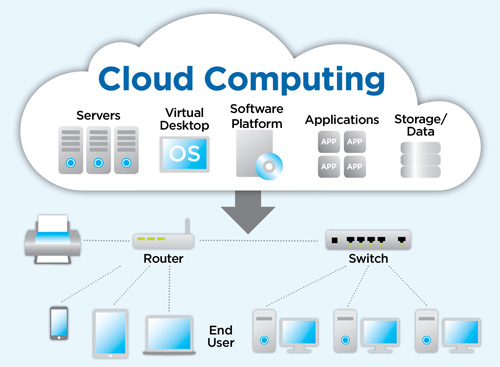
\includegraphics[scale=0.6]{figures/cloud-public.jpg}
	\caption{Architecture du Cloud}
	\label{cloud}
\end{figure}

\subsubsection{Sous-sous-sec1}
dsfsdf slkfj lsfj lkj lekj lzjeo fijzeif jzoiejf zoiej fozj efo
\subsubsection{Sous-sous-sec2}
Exemple de liste :

\begin{itemize}
	\item \textbf{Point 1}: azdpoakzd poakz poakz paokzd paokz 
	\item \textbf{Point 2}: csjc skjdc ksjd cksjc hskck s djc k
\end{itemize}
\subsection{Fog Computing}
azdazdazda a  jir iejrnf iejrnf ierjnf ierjn fiej ejnife
\section{Une autre section}
\lipsum[1-1] %genère un texte aléatoire
\chapter{Mon deuxième chapitre}
\section{Introduction}
\lipsum[1-1]%genère un texte aléatoire
\section{Une section}

\subsection{Une première sous-section}
\lipsum[1-1]%genère un texte aléatoire

\subsection{Une deuxième sous-section}
\lipsum[1-1]%genère un texte aléatoire

\subsubsection{Sous-sous-sec1}
\lipsum[1-1]%genère un texte aléatoire
\subsubsection{Sous-sous-sec2}

Exemple de liste :
\begin{itemize}
	\item \textbf{Point 1}: azdpoakzd poakz poakz paokzd paokz 
	\item \textbf{Point 2}: csjc skjdc ksjd cksjc hskck s djc k
\end{itemize}
\subsection{Fog Computing}
azdazdazda a  jir iejrnf iejrnf ierjnf ierjn fiej ejnife
\section{Une autre section}
\lipsum[1-1] %genère un texte aléatoire
\chapter{Mon troisième chapitre}
\section{Introduction}
\lipsum[1-1]%genère un texte aléatoire
\section{Une section}

\subsection{Une première sous-section}
\lipsum[1-1]%genère un texte aléatoire
\subsection{Une deuxième sous-section}
sdfkjdhfkjsdh fkjshd kfjh kjh zkejh kzjehf kjzhe kjeh fkjzhef

\subsubsection{Sous-sous-sec1}
zeflk zlek lkej flkzje flkzje flzkje flzkj flkzje flzkjfe lzkj
\subsubsection{Sous-sous-sec2}
Exemple de liste :

\begin{itemize}
	\item \textbf{Point 1}: azdpoakzd poakz poakz paokzd paokz 
	\item \textbf{Point 2}: csjc skjdc ksjd cksjc hskck s djc k
\end{itemize}
\subsection{Fog Computing}
azdazdazda a  jir iejrnf iejrnf ierjnf ierjn fiej ejnife
\section{Une autre section}
\lipsum[1-1] %genère un texte aléatoire
\chapter*{Conclusion générale et perspectives}
%\minitoc
% pour faire apparaître l'introduction dans le sommaire
\addcontentsline{toc}{chapter}{Conclusion générale et perspectives}

% Pour que l'entête soit correcte car chapter* ne redéfinit pas l'entête.
\lipsum[1-1]




\appendix
\chapter{Une annexe}

\lipsum[26-27]

 %inclure l'annexe si besoin

% bibliographie
\bibliography{allbiblio}
\end{document}%fin

